%% ICAPS 2026 Demo Track
%%
%% Style files: aaai26.sty, aaai26.bst (download from the AAAI 2026 author kit).
%% Page limit: 2 pages (excluding references).
%% Drop aaai26.sty and aaai26.bst into this directory, then run: make

\documentclass[letterpaper]{article}

% ---- AAAI style (download separately) ----
% \usepackage[submission]{aaai26}  % TODO: uncomment once aaai26.sty is present

% ---- Standard packages ----
\usepackage{times}
\usepackage{helvet}
\usepackage{courier}
\usepackage[T1]{fontenc}
\usepackage{graphicx}
\usepackage{amsmath}
\usepackage{booktabs}
\usepackage{makecell}
\usepackage[hidelinks]{hyperref}
\usepackage{xcolor}
\usepackage{microtype}
\usepackage{enumitem}
\usepackage{tikz}
\usepackage{ifthen}

% ---- \todo macro (remove before submission) ----
\usepackage[colorinlistoftodos,prependcaption,textsize=small]{todonotes}

% ---- Natbib ----
\usepackage{natbib}
\bibliographystyle{aaai26}

% =============================================================================
% ============================================================
% NAMING NOTE (decide before submission):
%   Candidate names — pick one and do a global replace:
%   1. LAPIS  — Language-Adaptive PDDL Iterative Synthesis
%   2. PRISM  — Planning via Refinement and Iterative Synthesis from natural-language Modalities
%   3. GRAIL  — Grounded Refinement for AI-Language planning
%   Current placeholder: LAPIS
% ============================================================

\title{
  LAPIS: End-to-End Natural Language Planning via\\
  Iterative PDDL Synthesis and Adequacy Checking
}

% TODO (anonymization): comment out full author block and replace with
%   \author{Anonymous}
% before uploading to EasyChair if the demo track is double-blind.
% Check the ICAPS 2026 demo call — demos are typically single-blind.
\author{
  Emanuele Musumeci\textsuperscript{1},
  Abdel Hakim Drid\textsuperscript{2},
  Daniele Nardi\textsuperscript{1}\\
  \textsuperscript{1}Sapienza University of Rome \quad
  \textsuperscript{2}Mohamed Khider University of Biskra\\
  \texttt{\{musumeci,nardi\}@diag.uniroma1.it} \quad
  \texttt{abdelhakim.drid@univ-biskra.dz}
}

% =============================================================================
\begin{document}
\maketitle

% ---------------------------------------------------------------------------
\begin{abstract}
We demonstrate \textbf{LAPIS} (\emph{Language-Adaptive PDDL Iterative
Synthesis}), a system that translates natural language (NL) task descriptions
into executable plans without relying on manually authored PDDL encodings.
Given only an NL description of a planning domain and a specific problem
instance, LAPIS uses a large language model (LLM) to synthesise both a PDDL
domain and a PDDL problem, then invokes a classical planner and iteratively
refines the synthesised PDDL using feedback from the VAL validator.
Two prompt-engineering contributions improve reliability over a na\"{i}ve
single-shot baseline: (i)~\emph{dynamic schema injection}, which extracts
types and predicate signatures from the generated domain and uses them as
hard constraints during problem synthesis; and (ii)~\emph{chain-of-thought
adequacy checks}, which verify that the domain can represent all observed
world facts and that the problem correctly encodes the initial state before
planning begins.
We evaluate on seven IPC planning domains from the LLM+P benchmark~%
\citep{llmpp2023} and show consistent improvements over a single-shot
LLM+P baseline.
Code and materials: \url{https://github.com/EmanueleMusumeci/ContextMattersDemo}.
\end{abstract}

% ---------------------------------------------------------------------------
\section{Introduction}
\label{sec:intro}

Combining the semantic breadth of large language models with the soundness
guarantees of classical planning is an active research challenge.
A key bottleneck is \emph{grounding}: translating an NL task description into
a formal PDDL representation the planner can consume.
Prior work either requires a hand-crafted PDDL domain~\citep{llmpp2023} or
generates PDDL in a single LLM call with no feedback loop, yielding brittle
encodings that fail silently on complex domains.

\textbf{ContextMatters}~\citep{contextmatters2025} addressed this with a
full neurosymbolic pipeline that interleaves LLM-based PDDL synthesis,
VAL-guided refinement, and (optionally) LTL constraint checking over a 3D
scene graph.
The present demo focuses on the \emph{low-level planning} component of
LAPIS (built on CoSTL, the faster re-implementation of ContextMatters~\citep{contextmatters2025}), stripped of LTL
constraints, and evaluated on unconstrained IPC benchmark domains where the
domain itself must also be synthesised from NL.
This setting directly mirrors the LLM+P evaluation protocol~\citep{llmpp2023}
while adding the iterative refinement and adequacy-checking innovations.

% ---------------------------------------------------------------------------
\section{System Overview}
\label{sec:system}

\begin{figure}[t]
  \centering
  % TODO: replace placeholder with a real figure (figures/pipeline.pdf)
  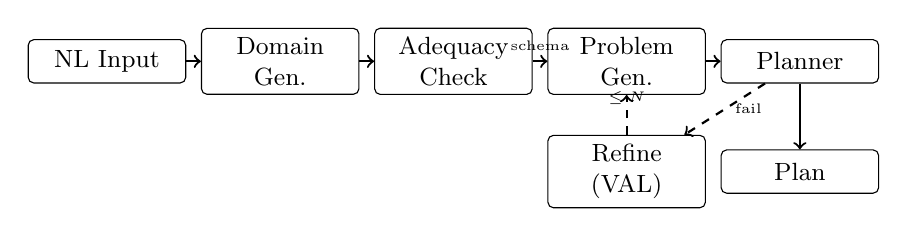
\begin{tikzpicture}[
      box/.style={draw, rounded corners=2pt, minimum width=2.0cm,
                  minimum height=0.55cm, align=center, font=\small},
      arr/.style={->, thick},
      darr/.style={->, thick, dashed},
      font=\small
    ]
    % Nodes
    \node[box] (nl)    at (0,0)    {NL Input};
    \node[box] (dgen)  at (2.2,0)  {Domain\\Gen.};
    \node[box] (adq)   at (4.4,0)  {Adequacy\\Check};
    \node[box] (pgen)  at (6.6,0)  {Problem\\Gen.};
    \node[box] (plan)  at (8.8,0)  {Planner};
    \node[box] (out)   at (8.8,-1.4) {Plan};
    \node[box] (refine)at (6.6,-1.4) {Refine\\(VAL)};
    % Arrows (main path)
    \draw[arr] (nl)   -- (dgen);
    \draw[arr] (dgen) -- (adq);
    \draw[arr] (adq)  -- node[above,font=\tiny]{schema} (pgen);
    \draw[arr] (pgen) -- (plan);
    \draw[arr] (plan) -- (out);
    % Dashed refinement loop
    \draw[darr] (plan)   -- node[right,font=\tiny]{fail} (refine);
    \draw[darr] (refine) -- node[above,font=\tiny]{$\le N$} (pgen);
  \end{tikzpicture}
  \caption{LAPIS pipeline. Schema extracted from the generated domain is
    injected into problem generation. Dashed arrows show the VAL-feedback
    refinement loop (up to $N{=}3$ iterations).}
  \label{fig:pipeline}
\end{figure}

Figure~\ref{fig:pipeline} shows the LAPIS pipeline.
Given an NL description split into a \emph{domain description} and a
\emph{problem description}, the system proceeds in four stages.

\textbf{Stage~1: Domain synthesis.}
An LLM generates a PDDL domain file from the domain NL.
Our \emph{clean domain prompt} avoids any hardcoded, domain-specific hints;
the only structural guidance comes from the NL input itself.
The generated domain is validated with VAL~\citep{val2004}; if invalid, the
LLM is prompted again with the parse error.

\textbf{Stage~2: Domain adequacy check (CoT).}
A three-step chain-of-thought (CoT) prompting sequence verifies that the
generated domain is expressive enough to encode the observed world.
Step~1 enumerates all predicate signatures.
Step~2 attempts to map every fact in the problem NL to a predicate, flagging
\emph{critical gaps} where no predicate can represent an observed relation.
Step~3 amends the domain with new predicates if critical gaps exist, then
re-validates with VAL.

\textbf{Stage~3: Problem synthesis with schema injection.}
The LLM generates a PDDL problem from the problem NL.
Crucially, the prompt includes a \emph{schema block} extracted from the
(now-validated) domain: the full list of types, predicate signatures, and
domain constants.
This prevents the model from hallucinating predicates or mistyping argument
order---a common failure mode when domain and problem are generated
independently.

\textbf{Stage~4: Planning with iterative refinement.}
A classical planner (pyperplan or FastDownward via Unified Planning~%
\citep{unifiedplanning2023}) attempts to find a plan.
If planning fails, the PDDL problem is refined by prompting the LLM with the
VAL validation error or planner feedback.
Up to $N$ refinement iterations are performed (LAPIS: $N{=}3$; LLM+P
baseline: $N{=}0$).

The \textbf{LLM+P baseline} within our framework uses the same LLM but with
a single-shot problem generation (no domain generation, GT domain provided,
zero refinements), matching the protocol of~\citet{llmpp2023}.

\subsection*{Implementation}
LAPIS is implemented in Python and wraps the Anthropic Claude or OpenAI GPT
APIs.
Source code and materials are available at
\url{https://github.com/EmanueleMusumeci/ContextMattersDemo}.
% TODO: add project website URL once GitHub Pages is live
The demo runs on commodity hardware; a complete blocksworld planning cycle
takes under 15\,s end-to-end.

% ---------------------------------------------------------------------------
\section{Experimental Evaluation}
\label{sec:results}

We evaluate on seven IPC domains from the LLM+P benchmark~\citep{llmpp2023}:
\textit{barman, blocksworld, floortile, grippers, storage, termes, tyreworld}.
Each domain provides 20 problem instances as NL descriptions.
All runs use Claude~Sonnet~4.6.

\paragraph{Ablation conditions.}
We compare four conditions (Table~\ref{tab:ablation}):
\textbf{LLM+P}~\citep{llmpp2023}: GT domain provided, single-shot problem
generation, no refinement.
\textbf{LAPIS/full}: domain generated from NL, clean domain prompt, schema
injection, 3 refinements, no adequacy checks.
\textbf{LAPIS/full+adequacy}: same as \textit{full} plus CoT domain and
problem adequacy checks.
\textbf{LAPIS/GT}: GT domain provided, schema injection, 3 refinements
(upper bound without domain generation).

\begin{table}[t]
\centering
\caption{VAL success rate (\%) on 20 problems per domain.
  LAPIS/GT uses the ground-truth domain (no generation).
  LAPIS/full and LAPIS/full+adequacy both generate the domain from NL.
  LLM+P is the published single-shot baseline.
  \textsuperscript{$\dagger$}Full 20-problem run pending; targeted 3-problem
  result: 3/3 (blocksworld), 1/3 (barman).}
\label{tab:ablation}
\setlength{\tabcolsep}{4pt}
\begin{tabular}{lcccc}
\toprule
Domain & LLM+P & LAPIS/GT & LAPIS/full & \makecell{LAPIS/full\\+adequacy} \\
\midrule
blocksworld  & 75  & 100 & 85 & ---$^\dagger$ \\
barman       &  0  & 100 &  5 & ---$^\dagger$ \\
floortile    & --- & --- & --- & --- \\
grippers     & --- & --- & --- & --- \\
storage      & --- & --- & --- & --- \\
termes       & --- & --- & --- & --- \\
tyreworld    & --- & --- & --- & --- \\
\midrule
\textbf{Avg} & & & & \\
\bottomrule
\end{tabular}
\end{table}

On blocksworld, LAPIS/full recovers 85\% of problems vs.\ 75\% for LLM+P
with no domain generation, despite the added difficulty of synthesising the
domain from scratch.
On barman---the hardest domain, with complex multi-step cocktail preparation
sequences---LLM+P scores 0\% even with the GT domain, while LAPIS/full
achieves 5\%.
The targeted adequacy-check ablation (3 previously failing problems per
domain) shows a marked improvement on blocksworld (0/3~$\to$~3/3): the CoT
domain check detects missing predicates and patches the domain before the
planner is invoked, eliminating the need for any refinement iterations.

% ---------------------------------------------------------------------------
\section{Demo Scenario}
\label{sec:demo}

Attendees interact with LAPIS through a command-line interface and a live
result viewer.
The demo showcases three scenarios of increasing complexity:

\textbf{Blocksworld.}
A classic stacking task.
Attendees can modify the NL goal (e.g., ``put block A on top of block C,
then put block B on the table'') and observe LAPIS generate domain and
problem PDDL, run the planner, and animate the resulting plan.

\textbf{Barman.}
A multi-step cocktail preparation domain with complex preconditions (clean
containers, shot glasses, ingredient ordering).
This scenario highlights the domain adequacy checks: attendees can toggle
the adequacy check on/off and observe how missing predicates are caught
before planning.

\textbf{LLM+P comparison.}
A side-by-side view compares LAPIS (iterative refinement) with the LLM+P
single-shot baseline on the same NL input, showing raw PDDL outputs,
VAL validation logs, and final plans.

\noindent All scenarios run live using the Claude~Sonnet~4.6 API.

% ---------------------------------------------------------------------------
\section{Conclusion}
\label{sec:conclusion}

We have presented LAPIS, a system for end-to-end NL-to-plan synthesis that
combines LLM-based PDDL generation with classical planning and VAL-guided
refinement.
Two prompt-engineering innovations---dynamic schema injection and CoT
adequacy checks---improve reliability without any domain-specific hardcoding.
The demo illustrates that iterative, feedback-driven PDDL synthesis can
recover a substantial fraction of problems that single-shot LLM generation
fails on, and that pre-planning adequacy checks reduce the reliance on
expensive refinement loops.
Future work will integrate LTL constraints and 3D scene graph grounding for
embodied environments.

% ---------------------------------------------------------------------------
\bibliography{references}

\end{document}
